%%implemenation 
This chapter specifies the approach taken to execute the project. Section~\ref*{codeoverview} gives an overview and 
describes the technologies used to carry out this project. Sections~\ref*{envsetup},~\ref*{stage1},~\ref*{stage2},~\ref*{stage3} 
explain how the program operates, and~\ref*{additions} provides information about some additional tooling developed to get better insight into the data. 
Section~\ref*{refactoring} provides an insight into the techniques used to refactor and optimise the orignal code~\cite{sftcdsur24:online}. 
The last section talks about the challenges faced during implementation.  

\section{Overview}
\label{codeoverview}
The program for surveying keys~\cite{sethr07s72:online} had various stages in which it performed different functions. Figure~\ref*{programstruct} depicts the flow of the program, and it can be divided into the following stages:
\begin{itemize}
    \item \textbf{Environment Setup:} Downloads all the required dependencies required for the program to work, including Python libraries, Maxmind databases, ZMap, ZGrab, and setups Golang.
    \item \textbf{Stage 1:} This stage can be called the Maxmind stage, where the MaxMind APIs are set up and filters out IP addresses for the country selected. 
    \item \textbf{Stage 2:} This is the scanning stage where ZMap and ZGrab are used. The IPs from Stage 1 are scanned using ZMap for open port 25. Once those IPs are available, ZGrab is used to capture data for the ports. 
    \item \textbf{Stage 3:} The final stage of the program where data from Stage 2 is processed, stored and analysis are carried out. 
\end{itemize}
\begin{figure}[h]
    \centering
    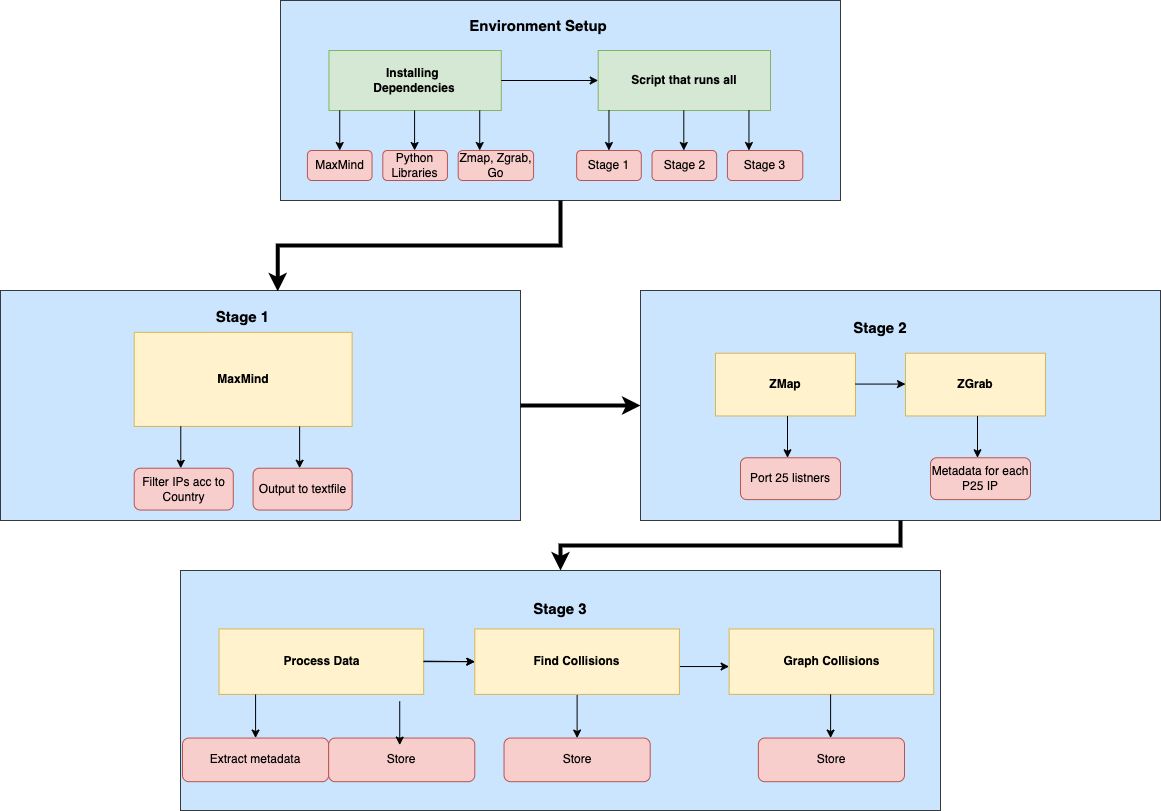
\includegraphics[width=18cm]{programstruct.drawio.png}
    \caption{Program Strcuture}
    \label{fig: Program Strcuture}
    \label{programstruct}
\end{figure}

\subsection{Technologies Used}
The following lists the technologies that were used to carry out the project:
\begin{itemize}
    \item \textbf{Python3:} Majority of the program was developed using Python3. Used for data processing, visualisation, and calling APIs and tools used.
    \item \textbf{Bash Script:} Used for automation of tasks, downloads and specific data extraction tasks.
    \item \textbf{ZMap:} Port scanner used to identity open port 25 listeners. 
    \item \textbf{ZGrab:} Banner Grabber to obtain information about hosts in question.
    \item \textbf{Maxmind:} Used databases and APIs provided by MaxMind to carry out the network scans.
    \item \textbf{Pylint:} A code analysis tool used to measure code quality and enforce a standard coding structure. 
    \item \textbf{cProfile and pstats:} A deterministic profiling tool used to optimise memory consumption and runtime.
\end{itemize}

\section{Environment Setup}
\label{envsetup}
Before the program execution begins, a script called \textit{``install-deps.sh''} downloads and installs all dependencies for the program to work. It starts by creating directories where the source code 
is available and another directory where the results for each scan are stored. After doing so, it will install dependencies like the Python libraries required, ZMap, ZGrab, and the MaxMind databases. 
It also installs Golang and configures the \textit{``gopath''} as ZGrab requires a valid \textit{``gopath''} to function. Since this program was the last run in 2018, the Maxmind databases have changed significantly. Therefore, 
an additional script called \textit{``MMIPs.py''} was developed to create a CSV dataset called \textit{``GeoIPCountryWhois''} was required for the program to run. The Python script takes in two CSV files as input that 
contain the entire IPv4 network blocks with their associated Geonames. In addition, there was another CSV file that had the Geonames and the country code and name associated. The script 
processes these two CSV files and then maps the IPv4 network blocks to their associated country code (and country names) using the Geonames. Finally, it produces the final CSV dataset needed.

\section{Stage 1: Maxmind Stage}
\label{stage1}
The program's first stage was to filter out the IP addresses for the country specificed to scan. For this project, the country choof interest was Ireland. 
The top script \textit{``skey-all.sh''} does all the work and calls these stages sequentially, as indicated in figure~\ref*{programstruct}. The script \textit{``IPsFromMM.py''} performs the first stage. 
It takes in the input file \textit{``GeoIPCountryWhois.csv''} and filters the IPv4 CIDRs according to the selected country. The final output from 
this stage is a text file that contains IPv4 CIDRs for the country chosen.

\section{Stage 2: Port Scan and Banner Grab}
\label{stage2}
This stage involved two parts. The first one was using ZMap to check for open port 25 listeners, and the next was using ZGrab on those hosts 
to gather the SSH and TLS meta-data.

\subsection{ZMap}
After getting the list of IPs for the country selected, the program moves onto the second stage and uses ZMap to map which IPs listen on port 25. ZMap is called 
using the main script \textit{``skey-all.sh''} as it requires system privileges. The final output from ZMap is a list of IP addresses that listen on port 25. 
Figure~\ref*{fig:zmapout} shows how the ZMap output looks like. It expands each IP in CIDR notation to the IP range and pings each IP in 
the range using the TCP SYN scan. The fields indicate the time left on the scan, the ``send: 2947'' shows that ZMap has pinged 2947 IPs address, 
and the ``recv:2'' means that ZMap has found two port 25 listeners. The ``hitrate: 0.07\%'' indicates that out of the total IPs pinged 0.07\%  
were port 25 listeners.  
\begin{figure}[h]
    \centering
    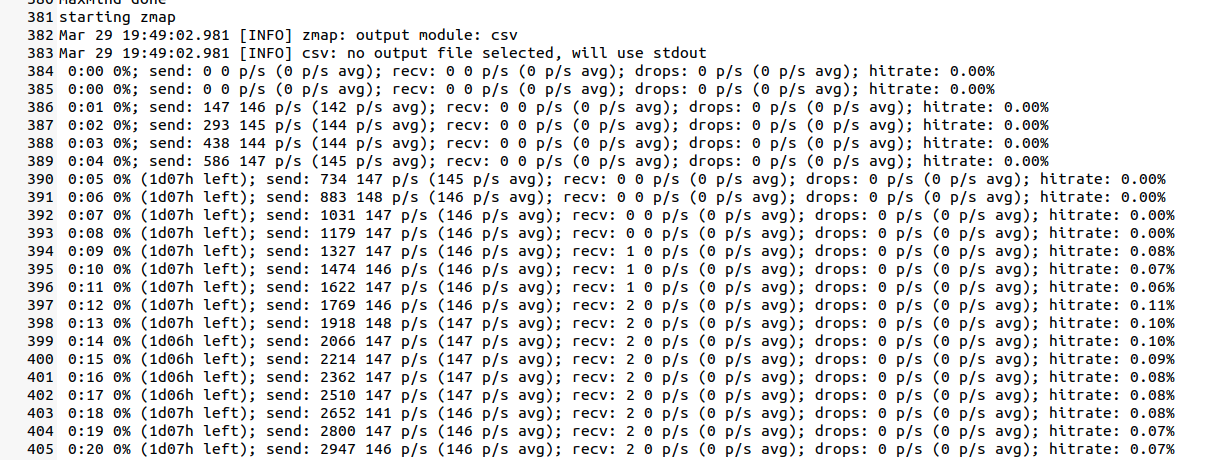
\includegraphics[width=18cm]{zmap_output.png}
    \caption{ZMap Output}
    \label{fig:zmapout}
\end{figure} 

\subsection{ZGrab}
The following process in this stage was to gather metadata about each port for IP addresses we obtained from ZMap. This is where the ZGrab2 tool was used, and the process was done using the script 
\textit{``FreshGrab.py''}. The script specifies the ZGrab parameters and calls the ZGrab binary. It requires an input file that is a list of IPs (ZMap output) and first verifies whether the IP belongs to the 
specified country using methods defined that make use of the Maxmind databases and APIs. If the IP does not match the country according to Maxmind, they are marked as ``out of country'' and are not processed further. 
The remaining IP addresses are processed using the ZGrab tool. Since the output is in JSON, the data is stored in a file called \textit{``records.fresh''} that 
contains one JSON structure per line. Each line has information about all seven ports for each IP. This part of Stage 2 can take anywhere 
from a few hours to a day to complete since the scan rate of the ZGrab tool was limited by adding a 100 ms wait between each IP so as not to cause any congestion in the network. 
\pagebreak

\begin{lstlisting}[caption={ZGrab2 Parameters}, captionpos=b, label={zgrabparams}]
    ports=['22', '25', '110', '143', '443', '587', '993']
    ztimeout=' -t 2'
    pparms={ 
        '22': 'ssh -p 22',
        '25': 'smtp -p 25 --starttls',
        '110': 'pop3 -p 110 --starttls',
        '143': 'imap -p 143 --starttls',
        '443': 'http -p 443 --use-https',
        '587': 'smtp -p 587 --smtps',
        '993': 'imap -p 993 --imaps',
        }
    for port in ports:
        cmd=zgrab_path + " " +  pparms[port] + ztimeout
        proc=subprocess.Popen(cmd.split(),stdin=subprocess.PIPE,stdout=subprocess.PIPE)
        pc=proc.communicate(input=ip.encode())
\end{lstlisting}

\noindent Listing~\ref*{zgrabparams} shows how ZGrab is used in the \textit{``FreshGrab.py''} script. The parameters specify the protocols and 
associated ports for it to scan for. To capture the TLS metadata for the plain text ports, the \textit{STARTTLS} command was used,
and implicit TLS for the other ports.

\section{Stage 3: Data Processing and Visualisation}
\label{stage3}
Stage 3 of the program involved parsing out the metadata from the JSON structures the project required, performing DNS and reverse DNS lookups, 
storing the data, and finding where the same key is being used for each IP for every possible host-port combination. Stage 3 can be broken down as follows:

\subsection{Data Processing}
The script that handles the data processing is \textit{``SameKeys.py''} and starts by iterating through data for each IP address in file \textit{``records.fresh''}. 
Since plenty of metadata is captured for each IP, the data is stored using Python, a class instance with multiple attributes. 
Then, the program starts by performing reverse DNS lookups for the IP and storing the names obtained in the same class instance. 
After that, Fully Qualified Domain Names, TLS certificates, and fingerprint information are parsed and stored for every port. 
The FQDNs are stored to assist with verifying the asset owners that are operating the said service. The program also keeps 
the information about the autonomous system associated with each host using the Maxmind databases. The methods to parse and store these 
fields are defined in the \textit{``SurveyFuncs.py''} script. Before moving onto the analysis stage, the program verifies names associated with the 
IPs by performing DNS lookups with the SANs related to the IP. The program only stored a maximum of 20 SANS per host, as some hosts have a large amount of SANs that 
slow down the program. If the IP addresses from the DNS lookup match the IP in \textit{``records.fresh''}, it is 
recorded as ``good''. Otherwise, it is recorded as ``bad''. The IPs marked as ``good'' with a key are stored in a JSON file for further analysis. 
The same is done with the ``bad'' IPs, and another file contains both IPs marked as both ``good'' and ``bad'' with their associated information. 
Appendix A provides the output of ZGrab and shows the information collected for all seven ports for each IP address. 
The appendix only provides data for one IP address in JSON format. 

\subsection{Data Analysis}
The data analysis process entails checking for the duplicate keys for different services within and across IPs. The clustering is based on fingerprint SHA-256 for each service. 
If a specific key is shared by two hosts irrespective of the protocol, they are put in the same cluster. This is because it is not uncommon to see key reuse for different services, as proved in~\cite{cryptoeprint:2018:299}. 
When key reuse is identified, the initial collisions are cross-checked with each other and are merged if the same key is being used there. 
Once, this is complete three files are produced as follows: 
\begin{itemize}
    \item ``collisions.json'': Contains key reuse information among hosts.
    \item ``dogies.json'': Contains information about IP that are recorded as ``bad''.
    \item  ``all-key-fingerprints.json'': Contains information that is included in the first two files. 
\end{itemize}

\subsection{Data Visualisation}
After obtaining the data as describe abovethe collisions are graphed using the Graphviz library in Python. The file used to graph the 
collisions is \textit{``collisons.json''}. Each host in the file is iterated through, and the hosts with the same cluster number are finally graphed using custom 
methods defined based on Graphviz.\\\\
\pagebreak
\begin{figure}[h!]
    \centering
    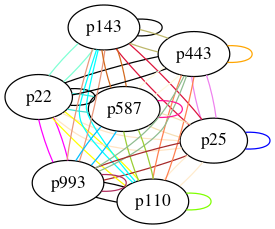
\includegraphics[width=11cm]{legend.png}
    \caption{Graph Legend}
    \label{fig:graphsleg}
\end{figure}

\noindent Figure~\ref*{fig:graphsleg} represents the graph legend, and the graphs can be visualised as follows:

\begin{itemize}
    \item The nodes are represented as IP addresses.
    \item The colour of the nodes represents the entities or hosts.
    \item The edges represent key reuse across ports. 
    \item The colour represents the pair port combination. 
\end{itemize}  

\section{Additional Tools}
\label{additions}
Some additional scripts are available that provide in-depth analysis of the data collected. For example, the script \textit{``ProtocolVersions.py''} 
provides an insight into the TLS/SSL versions seen throughout the scans and provides a count for them. It also provides details of 
the SSH versions seen on port 22. More tooling offers information on how many IP addresses were mapped by ZMap, how many host port 
combinations are there, how many unique fingerprints are seen, and many more. All of these scripts were used that assisted in the analysis of the results.

\section{Code Migration, Refactoring and Optimisation}
\label{refactoring}
One of the primary goals of this project was to migrate the code to Python3 and refactor it to increase readability, improve the structure, 
and optimise the run time and memory usage. This section gives details about the migration and the refactoring process. It also provides 
information about the techniques used to increase code performance.

\subsection{Code Refactoring}
The refactoring process was carried out by first analysing the entire program to check for duplicate code. Methods that were complex methods and involved heavy 
nesting were identified. In the \textit{``SameKeys.py''} script where the data processing takes place, all information parsing was done manually according 
to the JSON headers fields for each port. Due to this, the code was not so readable and looked complex. Therefore, the techniques 
outlined in section~\ref*{refactortechs} were used to carry out the refactoring. The following code snippets give an example of this. 

\begin{lstlisting}[caption={Code before Refactoring}, captionpos=b, label={codebefore}]
    try:
        p25=j_content['p25']
            if thisone.writer=="FreshGrab.py":
                banner=p25['data']['banner'] 
            else:
                banner=p25['smtp']['starttls']['banner'] 
            ts=banner.split()
            if ts[0]=="220":
                banner_fqdn=ts[1]
                nameset['banner']=banner_fqdn
            elif ts[0].startswith("220-"):
                banner_fqdn=ts[0][4:]
                nameset['banner']=banner_fqdn
    except Exception as e: 
        print >> sys.stderr, "FQDN banner exception " + str(e) + " for record:" + str(overallcount) + " ip:" + thisone.ip
        nameset['banner']=''
    try:
        if thisone.writer=="FreshGrab.py":
            tls=j_content['p25']['data']['tls']
            cert=tls['server_certificates']['certificate']
        else:
            tls=j_content['p25']['smtp']['starttls']['tls']
            cert=tls['certificate']
            fp=cert['parsed']['subject_key_info']['fingerprint_sha256'] 
            get_tls(thisone.writer,'p25',tls,j_content['ip'],thisone.analysis['p25'],scandate)
            get_certnames('p25',cert,nameset)
            thisone.fprints['p25']=fp
            somekey=True
    except Exception as e: 
        print >> sys.stderr, "p25 exception for:" + thisone.ip + ":" + str(e)
        pass   
\end{lstlisting}
\begin{lstlisting}[caption={Code After Refactoring}, captionpos=b, label={codeafter}]
    try:
        p25 = j_content['p25']
        bn = "y"
        if thisone.writer == "FreshGrab.py":
            banner_fqdn = get_mail_data(p25, bn)
        else:
            banner = p25['smtp']['starttls']['banner']
            nameset['banner'] = banner_fqdn
    except Exception as e:
        print(sys.stderr, "FQDN banner exception " + str(e) + " for record:" + str(overallcount) + " ip:" + thisone.ip)
        nameset['banner'] = ''
    try:
        if thisone.writer == "FreshGrab.py":
            data = j_content['p25']['data']['smtp']['result']['tls']
            cert, fp = get_mail_data(data, None)
        else:
            tls = j_content['p25']['smtp']['starttls']['tls']
            cert = tls['certificate']
        get_tls(thisone.writer, 'p25', data, j_content['ip'], thisone.analysis['p25'], scandate)
        get_certnames('p25', cert, nameset)
        thisone.fprints['p25'] = fp
        somekey = True
    except Exception as e:
        print (sys.stderr, "p25 exception for:" + thisone.ip + ":" + str(e))
        pass
\end{lstlisting}
Listing~\ref*{codebefore} and Listing~\ref*{codeafter} shows the code before and after refactoring respectively. In this instance, a method 
was introduced called \verb|get_mail_data(data,banner)| that was used to extract the banner information for port 25, but also to gather 
the TLS certificate and fingerprint data for all mail protocols instead of doing this manually for each mail port.\\
Other methods were created as well, and the existing ones were modified for simplicity. This was done to decrease the number of 
lines of code in the \textit{``SameKeys.py''} script and to avoid writing duplicate code. It also had another benefit that in case there 
are changes to the ZGrab output in the future, one will have to make changes in the program at one point instead of doing it manually 
for all ports.\\\\
Another instance where refactoring was carried out was in the \textit{``SurveyFuncs.py''} script that contains custom utility functions. 
While it is still somewhat acceptable to have manual code in this script as it is not used directly, refactoring was carried out here 
to improve performance. For example, existing methods that were used to call the Maxmind APIs contained a lot of nesting of \textit{if} 
statements and \textit{for} loops. To decrease the nesting, the abstraction technique was used to break down the nested statements by defining 
different methods to perform the same function overall. 

\subsection{Code Optimisation}
To optimise this program, memory analysis had to be carried out that gave information about the memory overheads of the program and identified what was 
taking the most amount of time to complete the whole process. This analysis was carried out using the \textit{cProfile} and \textit{pstats} 
libraries available in open-source. A profile here is defined as a ``set of statistics that describes how often and for how long various parts 
of the program are being executed''~\cite{ThePytho56:online}. When used with the scripts, this library gives a detailed report about how the program behaves. 
It gives information about the number of monitored calls and how many of those were primitive or recursive. In addition, it provides the total time spent 
in each method and the cumulative time spent in the method and all sub-methods. Once this data was available, it was investigated, and areas of the program were 
identified where bottlenecks were being created. Finally, alternative solutions were explored to decrease run time and to decrease memory usage.
\newpage

\begin{figure}[h!]
    \centering
    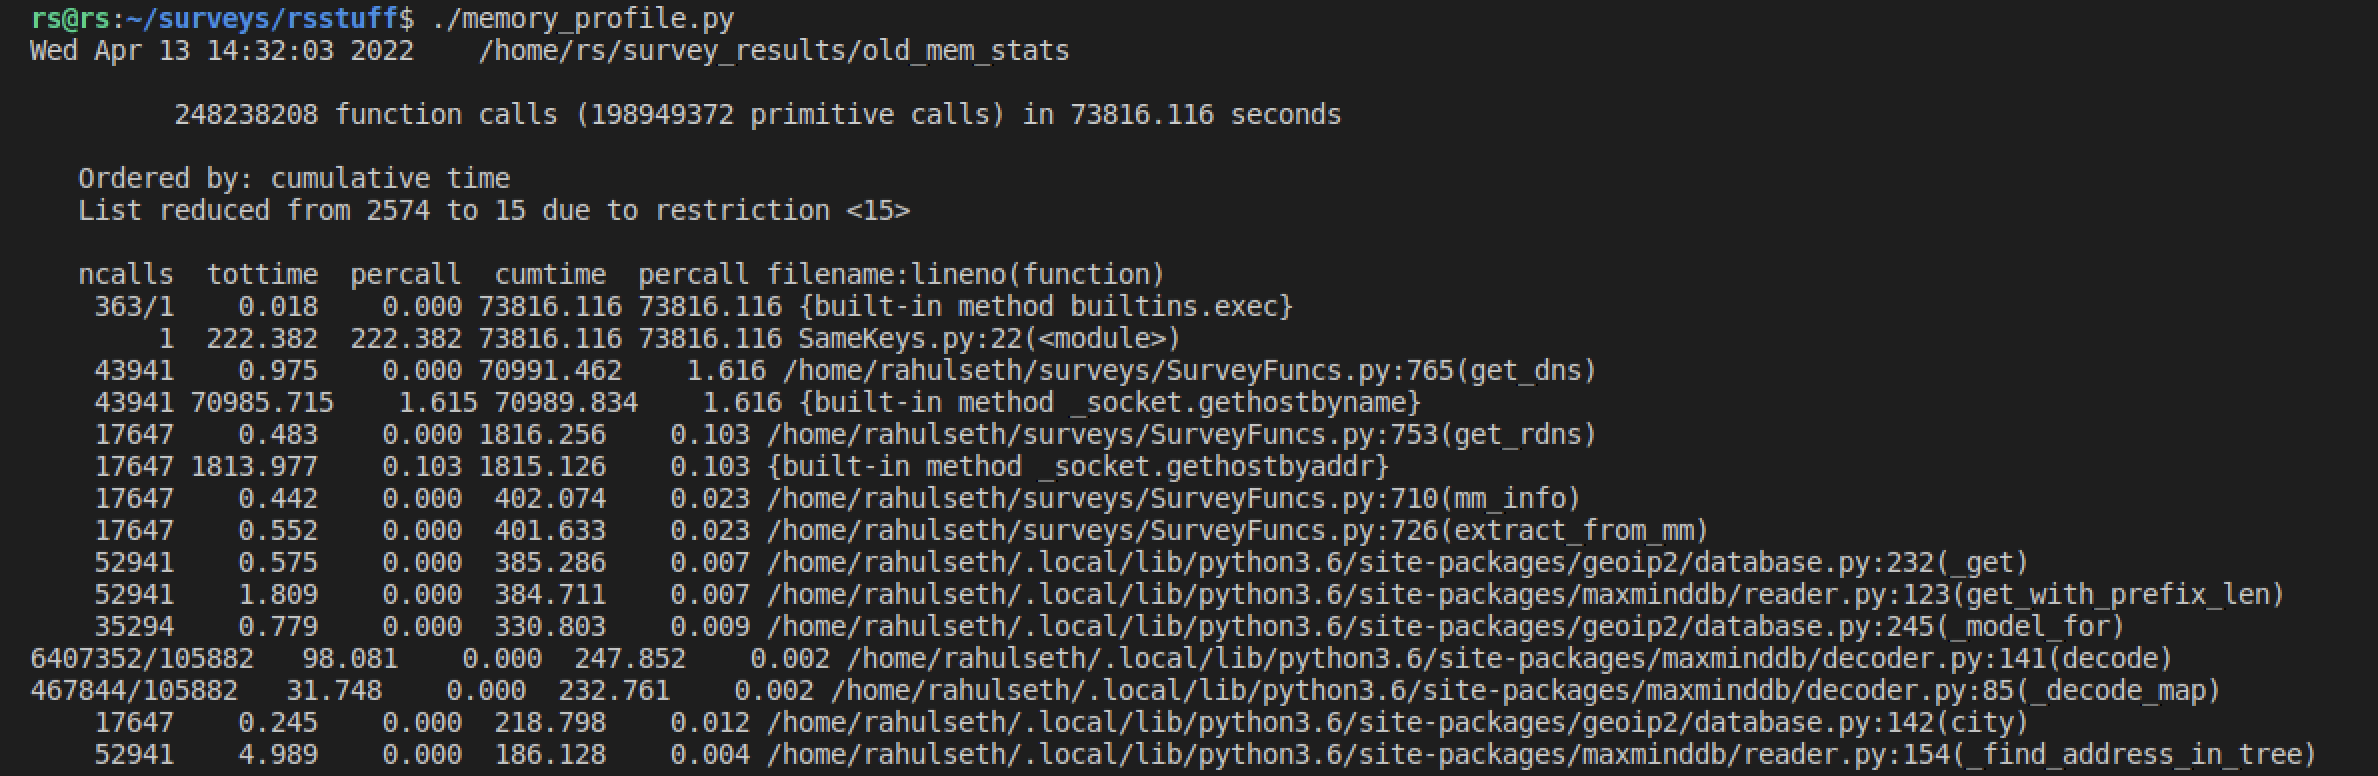
\includegraphics[width=18cm]{old_mem_profile.png}
    \caption{Memory Profile before Refactoring}
    \label{fig:oldmemprof}
\end{figure}

\noindent Figure~\ref*{fig:oldmemprof} depicts the output upon profiling the code before any optimisation or major refactoring was carried out. 
The above profiling was done on the same data that was used to carry out the data analysis. Referring to the figure, it is visible the total 
execution time of the program was about 73816 seconds, but most of the time was consumed by the function \verb|gethostbyname()| that is 
used to perform DNS lookups on the names parsed out from the metadata. The names include banner information and 
subject alternative names (SANs). Once this bottleneck was identified, alternative DNS resolution solutions were looked at 
(discussed in the section below), and different benchmark tests were created in order to see the timing of each solution and which met the 
scope of the project.

\subsection{DNS Resolving}
After memory profiling the program, it was found that the DNS resolution part of the code was consuming much time. Few alternate solutions 
were explored for faster resolution to decrease the run time. Reasons why DNS resolution was creating a bottleneck were investigated. 
Some solutions that were looked at to mitigate this problem were: DNSpython, MassDNS Resolver, Berserker Resolver, and Stubby plus Unbound. 
A benchmark timing test was created for the four, and it was found that using a combination of stubby plus unbound was the fastest among them. 
The problem with the first three options were as follows: 
\begin{itemize}
    \item MassDNS~\cite{blechsch83:online} is used to make queries in the range of millions to billions and was not fitting the scope of the project. 
    \item DNSpython~\cite{dnspytho38:online} had the same performance as \verb|gethostbyname()| function in the socket library 
    unless a timeout value was set for lookups which was not the most efficient way to solve this issue.
    \item Berserker Resolver~\cite{berserke53:online} had an upgrade in performance but used DNSpython in the backend. 
\end{itemize} 
A more permanent solution was required, and that was using a combination of two open-source tools called Unbound and Stubby. Unbound is a 
validation, recursive, caching DNS resolver that is designed to be fast and lean and provides modern services like DNS over TLS and DNS over HTTPS, 
which allows encryption while making name resolutions~\cite{NLnetLab67:online}. Stubby is an application that acts as a local DNS stub 
resolver and uses DNS-over-TLS for resolutions. The combination of Unbound and Stubby was used to speed up the DNS resolution for our program.\\ 
Unbound was used behind stubby, and all queries made using Unbound were forwarded to Stubby. Since Stubby uses DNS over TLS, which is assigned to port 853 as compared to 
traditional DNS that operates on port 53. The configuration had to be set up for the same. Before testing the code with this combination, 
Wireshark was used to analyse the traffic on port 853 while performing DNS lookups to ensure it was functioning as expected. 
Wireshark is a network packet analyser that captures in-depth detail about the captured packet~\cite{Chapter148:online}.
\newpage

\section{Challenges}
\label{challenges}
This project came across a few expected challenges. One of the significant challenges was configuring and visualising the ZMap and ZGrab tools. Although it was relatively 
easy to understand how ZMap works and how the output would look, the ZGrab posed a real challenge since the output from the tool was in JSON and involved heavy nesting.
Development for this program was done using various Linux systems, and the table below shows the Virtual Machines that were set up and 
their purpose during the course of this project.

\begin{table}[h!]
    \centering
    \begin{tabular}{|c|c|}
        \hline
        Ubuntu Version  &   Purpose\\
        \hline
        22.04   &   Development \\
        \hline
        21.04   &   Target VM for testing ZGrab\\
        \hline
        18.04   &   Testing\\
        \hline
    \end{tabular}
    \caption{VM Setup}
    \label{vm:vmsetup}

    \quad
    
    \begin{tabular}{|c|c|}
        \hline
        Service  &   Protocol\\
        \hline
        Apache Server   &   HTTPS,SSH\\
        \hline
        Dovecot   &   IMAP and POP3\\
        \hline
        Postfix   &   SMTP\\
        \hline
    \end{tabular}
    \caption{Target VM Setup}
    \label{tab:targetvmsetup}
\end{table}

\noindent The target VM was set up with different servers available in open-source that offered the protocols required. Table~\ref*{tab:targetvmsetup} 
shows the server setup on the target VM and the protocols provided by each. These servers were set up using minimal configurations to test the ZGrab 
tool over localhost. Since the program used a Python Script to use the ZGrab tool and performed IP checks according to the MaxMind databases, 
the reserved IP addresses could not be used as MaxMind does not recognise them as it operates the same blacklist as ZMap. 
Due to this, the ZGrab tool was tested manually using the command-line interface for each protocol by adding multiple IPv4 addresses and mapping 
them to each service configured.




